\documentclass[11pt,a4paper]{article}

\usepackage[T1]{fontenc}
\usepackage[utf8]{inputenc}
\usepackage[english]{babel}
\usepackage{amsmath,amssymb,mathtools}
\usepackage{geometry}
\usepackage{graphicx}
\usepackage{booktabs}
\usepackage{hyperref}
\usepackage{enumitem}
\usepackage{float}

\geometry{margin=2.5cm}
\emergencystretch=2em

\hypersetup{
  colorlinks=true,
  hypertexnames=false,
  linkcolor=blue,
  citecolor=blue,
  urlcolor=blue
}

\graphicspath{
  {outputs_paper45/}
  {../experiments/maat_metric_response_paper45/outputs_paper45/}
}

\newcommand{\LCDM}{\Lambda\mathrm{CDM}}
\newcommand{\Chatproj}{\widehat{\mathcal{C}}_{\mathrm{proj}}}
\newcommand{\fsig}{f\sigma_8}
\newcommand{\Geff}{G_{\mathrm{eff}}}
\newcommand{\etaslip}{\eta_{\mathrm{slip}}}

\title{
\textbf{Effective Metric Response in MAAT Structural Cosmology}\\[0.4em]
\large Gravitational Slip, Weyl-Potential Proxies, and Growth--Lensing Consistency
}

\author{
Christof Krieg\\
\small MAAT Project -- Independent Research\\
\small \url{https://maat-research.com}
}

\date{2026}

\begin{document}

\maketitle

\begin{abstract}
Previous MAAT cosmology papers promoted the structural projection observable
from a diagnostic quantity to an effective source for linear matter growth.
In Paper 43, this was implemented through a bounded projection kernel
$\Chatproj(z)$ entering the growth coupling
$\mu(z)=\Geff/G=1+\eta_g\Chatproj(z)$.
The resulting benchmark closed the first explicit growth-ODE layer, but it did
not yet address metric perturbations, gravitational slip, or lensing-sensitive
combinations of the scalar potentials.

This paper introduces a minimal effective metric-response benchmark.
Working in the Newtonian-gauge scalar-potential language, we supplement the
growth coupling by a gravitational-slip relation
\[
\etaslip(z)=\frac{\Phi}{\Psi}=1+\beta_s\Chatproj(z),
\]
and define the Weyl/lensing response
\[
\Sigma(z)=\mu(z)\frac{1+\etaslip(z)}{2}.
\]
This extends the MAAT perturbative pipeline from growth response to metric
response while remaining an effective, bounded, non-Boltzmann-code test.

Numerically, we scan
$\eta_g\in[0,0.08]$ and $\beta_s\in[-0.06,0.06]$, giving $2501$ metric-response
branches.
All scanned branches remain positive and stable in the tested sense.
The compact growth-only comparison still prefers the $\LCDM$ limit
$\eta_g=0$, while $\beta_s$ is unconstrained without lensing data.
For a representative nonzero branch
$(\eta_g,\beta_s)=(0.02,0.03)$, the maximum deviations over $0\le z\le3$ are
$|\mu-1|\simeq1.997\%$, $|\etaslip-1|\simeq2.995\%$,
$|\Sigma-1|\simeq3.524\%$, and a Weyl-proxy deviation of
$\simeq2.731\%$.

The contribution is methodological: MAAT structural projection can be embedded
into the standard metric-response language of linear cosmological
perturbations without producing immediate pathologies.
The result is not a weak-lensing likelihood, a CMB calculation, or evidence for
modified gravity.
\end{abstract}

\section{Purpose and Status}

Paper 43 established the first explicit MAAT linear-growth equation by
embedding the bounded projection kernel $\Chatproj(z)$ into the effective
growth coupling $\mu(z)$.
This was a necessary but incomplete perturbative step.
Growth data probe matter clustering, but relativistic cosmology also probes
the scalar metric potentials through lensing, integrated Sachs--Wolfe effects,
and growth--lensing consistency.

The purpose of the present paper is therefore:
\begin{quote}
\emph{to extend MAAT structural cosmology from growth-only response to a
minimal effective metric-response benchmark.}
\end{quote}

The status is deliberately conservative.
This paper does not implement a Boltzmann solver, does not compute CMB
anisotropies, does not include weak-lensing likelihoods, and does not claim a
precision cosmological fit.
It provides a reproducible bridge from the MAAT projection layer to the
standard $\mu$--$\Sigma$--slip language used in phenomenological tests of
gravity.

\section{Background: Scalar Metric Potentials}

In Newtonian gauge, scalar perturbations of a spatially flat FLRW background
can be written schematically as
\begin{equation}
ds^2
=
-(1+2\Psi)\,dt^2
+
a^2(t)(1-2\Phi)\delta_{ij}dx^i dx^j .
\end{equation}
In minimally coupled general relativity with negligible anisotropic stress,
\begin{equation}
\Phi=\Psi.
\end{equation}
Many effective modified-gravity parameterizations instead introduce two
functions:
\begin{align}
k^2\Psi
&=
-4\pi G a^2 \mu(a)\rho_m\delta_m,\\
\Phi
&=
\etaslip(a)\Psi.
\end{align}
The combination relevant for weak lensing is the Weyl potential
$\Phi+\Psi$.
It is conventional to define
\begin{equation}
k^2(\Phi+\Psi)
=
-8\pi G a^2 \Sigma(a)\rho_m\delta_m,
\end{equation}
where
\begin{equation}
\Sigma(a)
=
\mu(a)\frac{1+\etaslip(a)}{2}.
\label{eq:sigma_def}
\end{equation}
Thus $\Sigma$ parameterizes the Weyl/lensing response channel: it measures how
the lensing potential responds relative to the matter density contrast.

\section{MAAT Metric-Response Ansatz}

The bounded projection kernel is inherited from Paper 43:
\begin{equation}
\Chatproj(z)
=
\frac{
\mathcal{C}_{\mathrm{proj}}(z)-\mathcal{C}_{\mathrm{proj}}(0)
}{
\mathcal{C}_{\mathrm{proj}}(z_{\max})-\mathcal{C}_{\mathrm{proj}}(0)
},
\qquad
0\le\Chatproj(z)\le1,
\label{eq:chat}
\end{equation}
with $z_{\max}=3$ in the present benchmark.

The growth response remains
\begin{equation}
\mu(z)
=
1+\eta_g\Chatproj(z),
\label{eq:mu}
\end{equation}
where $\eta_g$ controls the maximum fractional change of the effective
Newtonian growth coupling over the tested interval.

The new metric-response ingredient is the slip ansatz
\begin{equation}
\etaslip(z)
=
\frac{\Phi}{\Psi}
=
1+\beta_s\Chatproj(z),
\label{eq:slip}
\end{equation}
where $\beta_s$ controls the maximum slip deformation.
Operationally, a nonzero slip corresponds to an effective anisotropic-stress
sector in the metric perturbations, even though no microscopic anisotropic
stress model is derived here.
Combining Eqs.~\eqref{eq:sigma_def}--\eqref{eq:slip} gives
\begin{equation}
\Sigma(z)
=
\left[1+\eta_g\Chatproj(z)\right]
\left[
1+\frac{\beta_s}{2}\Chatproj(z)
\right].
\label{eq:sigma_maat}
\end{equation}

This construction is not interpreted as a fundamental variation of Newton's
constant.
It is an effective metric-response insertion of the same structural projection
kernel already used in the growth sector.

\section{Growth Equation}

The matter growth equation is the same as in Paper 43:
\begin{equation}
\frac{d^2D}{dN^2}
+
\left[
2+\frac{d\ln H}{dN}
\right]
\frac{dD}{dN}
-
\frac32\Omega_m(a)\mu(a)D
=0,
\label{eq:growth}
\end{equation}
where $N=\ln a$ and $D(a)$ is normalized to $D(a=1)=1$.
For $\eta_g=0$, Eq.~\eqref{eq:growth} reduces to the $\LCDM$ reference growth
equation.

The growth observable is
\begin{equation}
\fsig(z)
=
f(z)D(z)\sigma_{8,0},
\qquad
f=\frac{d\ln D}{d\ln a}.
\end{equation}
The compact $\fsig$ comparison set used in Papers 40, 42, and 43 is reused
only to quantify the growth channel.
It does not constrain $\beta_s$, because $\beta_s$ enters the metric/lensing
sector rather than the growth equation.
Equivalently, the source term of Eq.~\eqref{eq:growth} depends on $\mu(z)$,
not on $\etaslip(z)$; the slip channel becomes observable only through
metric-potential probes such as lensing or ISW-type measurements.

\section{Lensing and Consistency Proxies}

Because this benchmark does not implement a weak-lensing likelihood, we report
two diagnostic proxies rather than data-level observables.
The first is a Weyl-amplitude proxy,
\begin{equation}
W_{\mathrm{proxy}}(z)
=
\Sigma(z)\frac{D_{\mathrm{MAAT}}(z)}{D_{\LCDM}(z)}.
\label{eq:weyl_proxy}
\end{equation}
The second is an $E_G$-like growth--lensing consistency proxy,
\begin{equation}
E_{G,\mathrm{proxy}}(z)
=
\Sigma(z)\frac{f_{\LCDM}(z)}{f_{\mathrm{MAAT}}(z)}.
\label{eq:eg_proxy}
\end{equation}
These quantities are not replacements for lensing maps or galaxy--lensing
cross-correlations.
They are diagnostic projections showing how the metric-response layer would
separate growth and lensing channels.

\section{Numerical Setup}

The benchmark uses the same Planck-like flat $\LCDM$ reference and projection
parameters as Paper 43:
\begin{align}
H_0 &= 67.4\;\mathrm{km\,s^{-1}\,Mpc^{-1}},\\
\Omega_{m0} &= 0.315,\\
\Omega_{\Lambda0} &= 0.685,\\
\sigma_{8,0} &= 0.811.
\end{align}

The scan ranges are
\begin{equation}
\eta_g\in[0,0.08],
\qquad
\beta_s\in[-0.06,0.06],
\end{equation}
with $41$ values of $\eta_g$ and $61$ values of $\beta_s$.
This gives $2501$ metric-response branches.

The representative nonzero branch used in the figures is
\begin{equation}
\eta_g=0.02,
\qquad
\beta_s=0.03.
\end{equation}
The stability checks are deliberately minimal:
\begin{equation}
\mu(z)>0,
\qquad
\etaslip(z)>0,
\qquad
\Sigma(z)>0,
\qquad
D(z)>0,
\qquad
f(z)>0.
\end{equation}

\section{Results}

\begin{table}[H]
\centering
\caption{Paper 45 metric-response scan summary.}
\begin{tabular}{lr}
\toprule
\textbf{Quantity} & \textbf{Value} \\
\midrule
$\eta_g$ scan & $[0.00,0.08]$ with $41$ points \\
$\beta_s$ scan & $[-0.06,0.06]$ with $61$ points \\
Total branches & $2501$ \\
Stable / positive branches & $2501/2501$ \\
Growth-only best $\eta_g$ & $0.0000$ \\
Growth-only $\beta_s$ & unconstrained without lensing data \\
Best growth-only $\chi^2$ & $12.2021$ \\
\bottomrule
\end{tabular}
\end{table}

The growth-only compact comparison again prefers the $\LCDM$ limit
$\eta_g=0$.
This is consistent with Paper 43.
The slip parameter $\beta_s$ is not constrained by the growth-only comparison,
which is exactly why metric or lensing information is needed.

\begin{table}[H]
\centering
\caption{Representative nonzero branch, $\eta_g=0.02$, $\beta_s=0.03$.}
\begin{tabular}{lr}
\toprule
\textbf{Quantity} & \textbf{Maximum absolute deviation for $0\le z\le3$} \\
\midrule
$|\Delta D/D|$ & $0.7656\%$ \\
$|\Delta\fsig/\fsig|$ & $0.5441\%$ \\
$|\mu-1|$ & $1.9966\%$ \\
$|\etaslip-1|$ & $2.9949\%$ \\
$|\Sigma-1|$ & $3.5240\%$ \\
Weyl-proxy deviation & $2.7314\%$ \\
$E_G$-proxy deviation & $2.3019\%$ \\
\bottomrule
\end{tabular}
\end{table}

\begin{figure}[H]
\centering
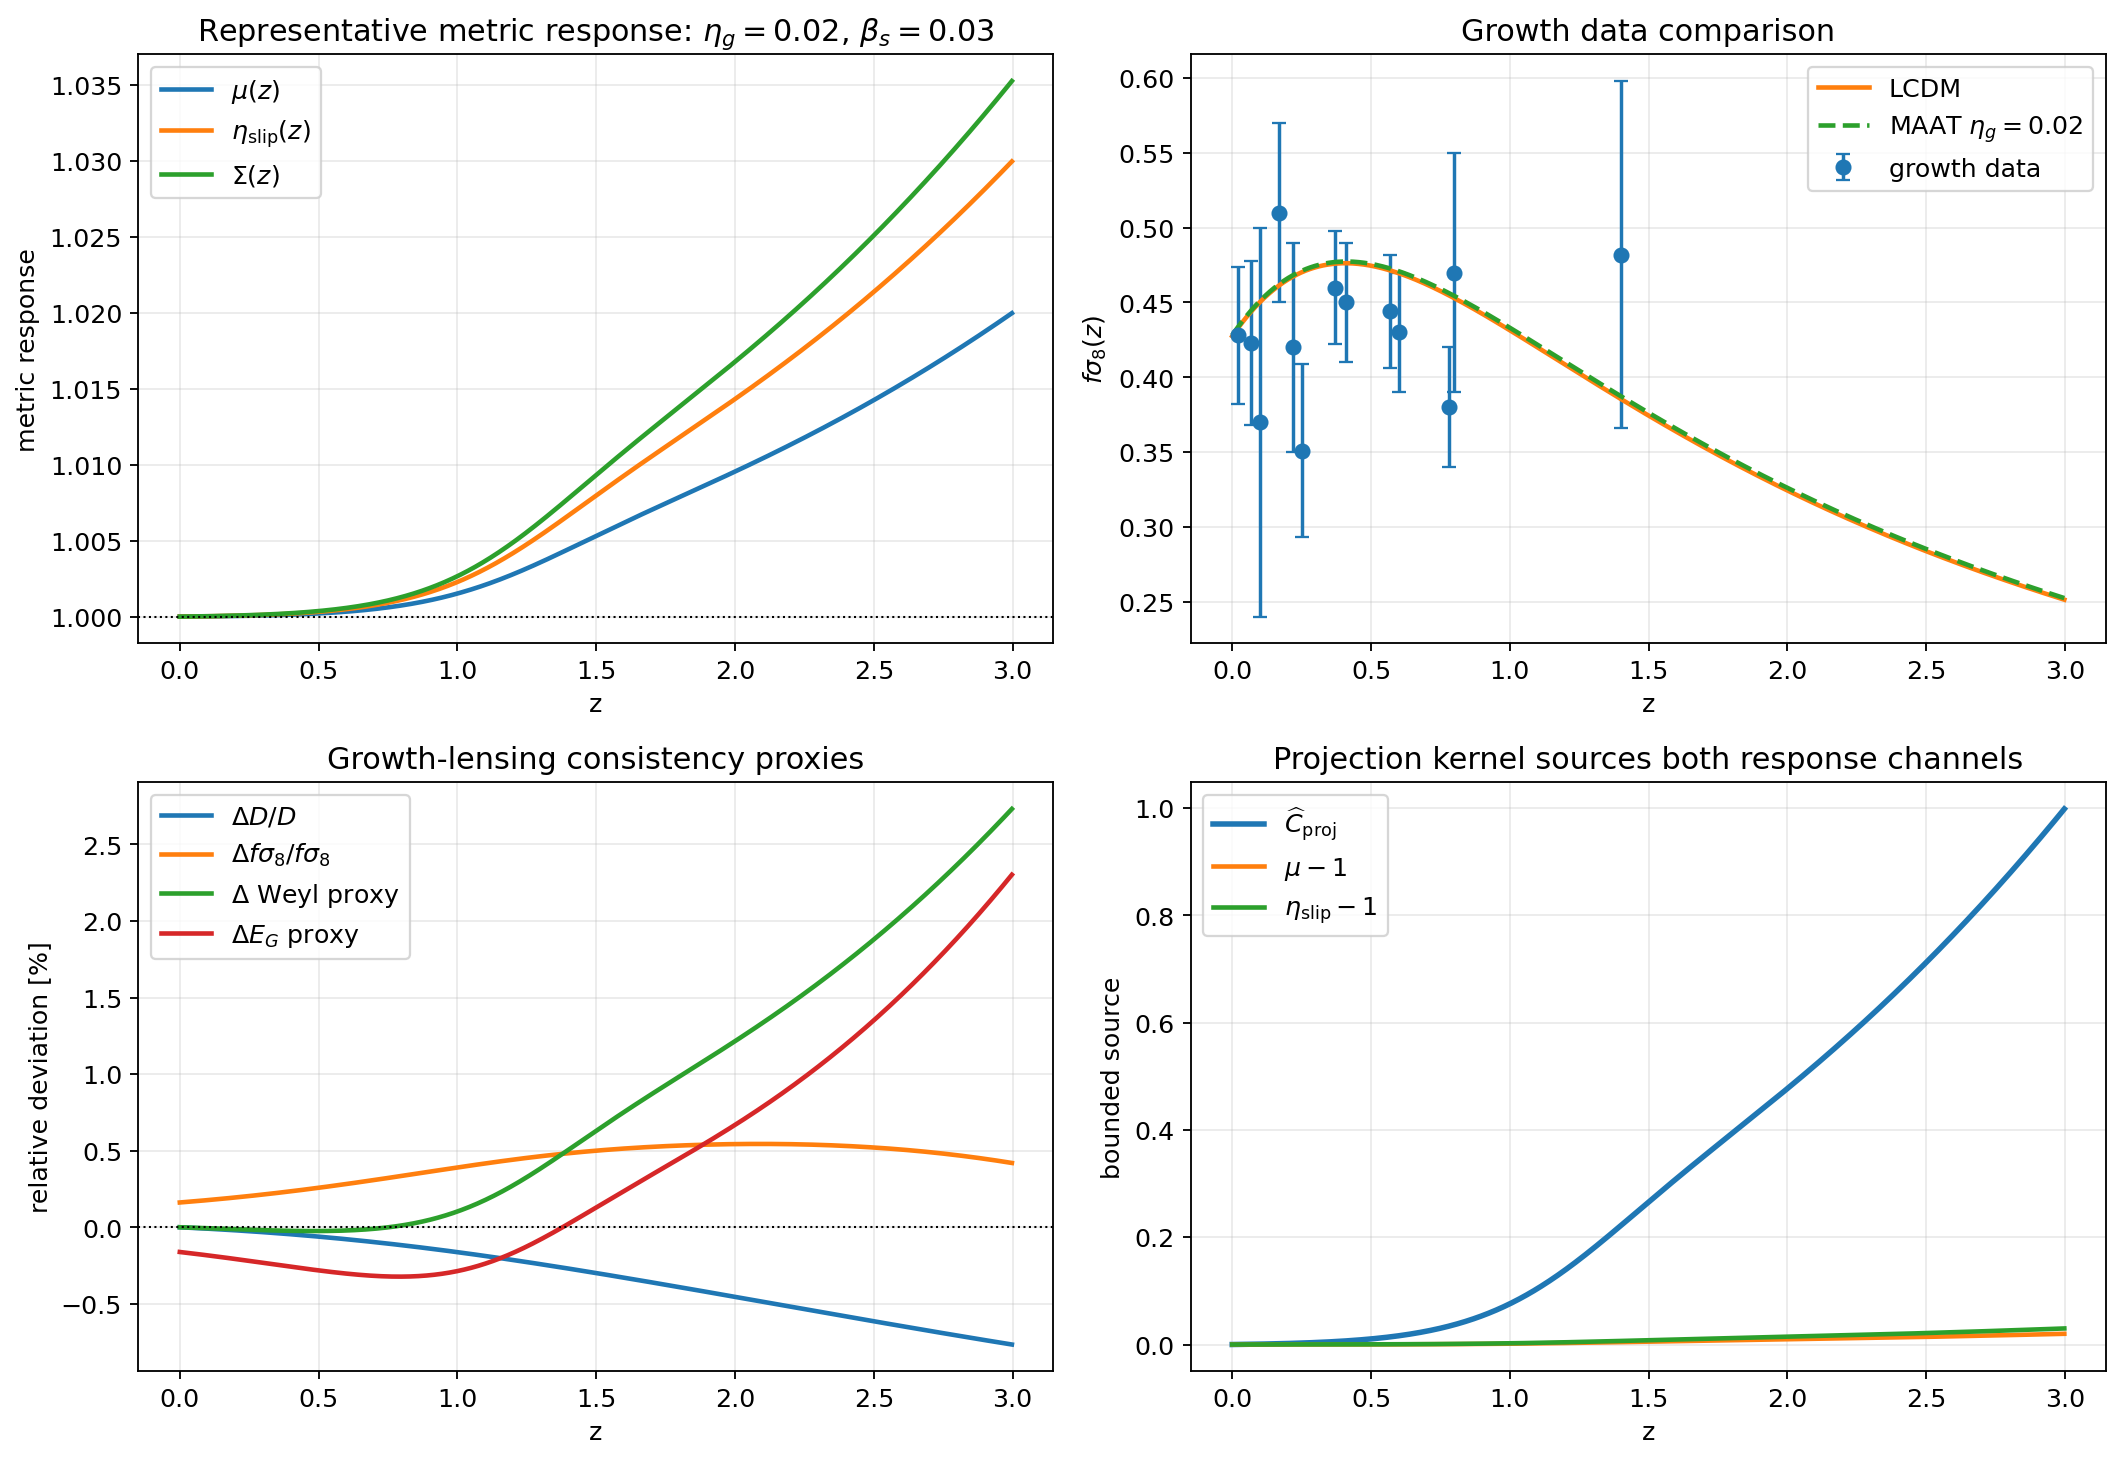
\includegraphics[width=0.96\linewidth]{fig1_metric_response_summary.png}
\caption{Paper 45 metric-response summary.
Top left: representative metric response functions.
Top right: compact $\fsig$ comparison.
Bottom left: growth, Weyl, and $E_G$ proxy deviations.
Bottom right: bounded projection kernel sourcing both response channels.}
\label{fig:summary}
\end{figure}

\begin{figure}[H]
\centering
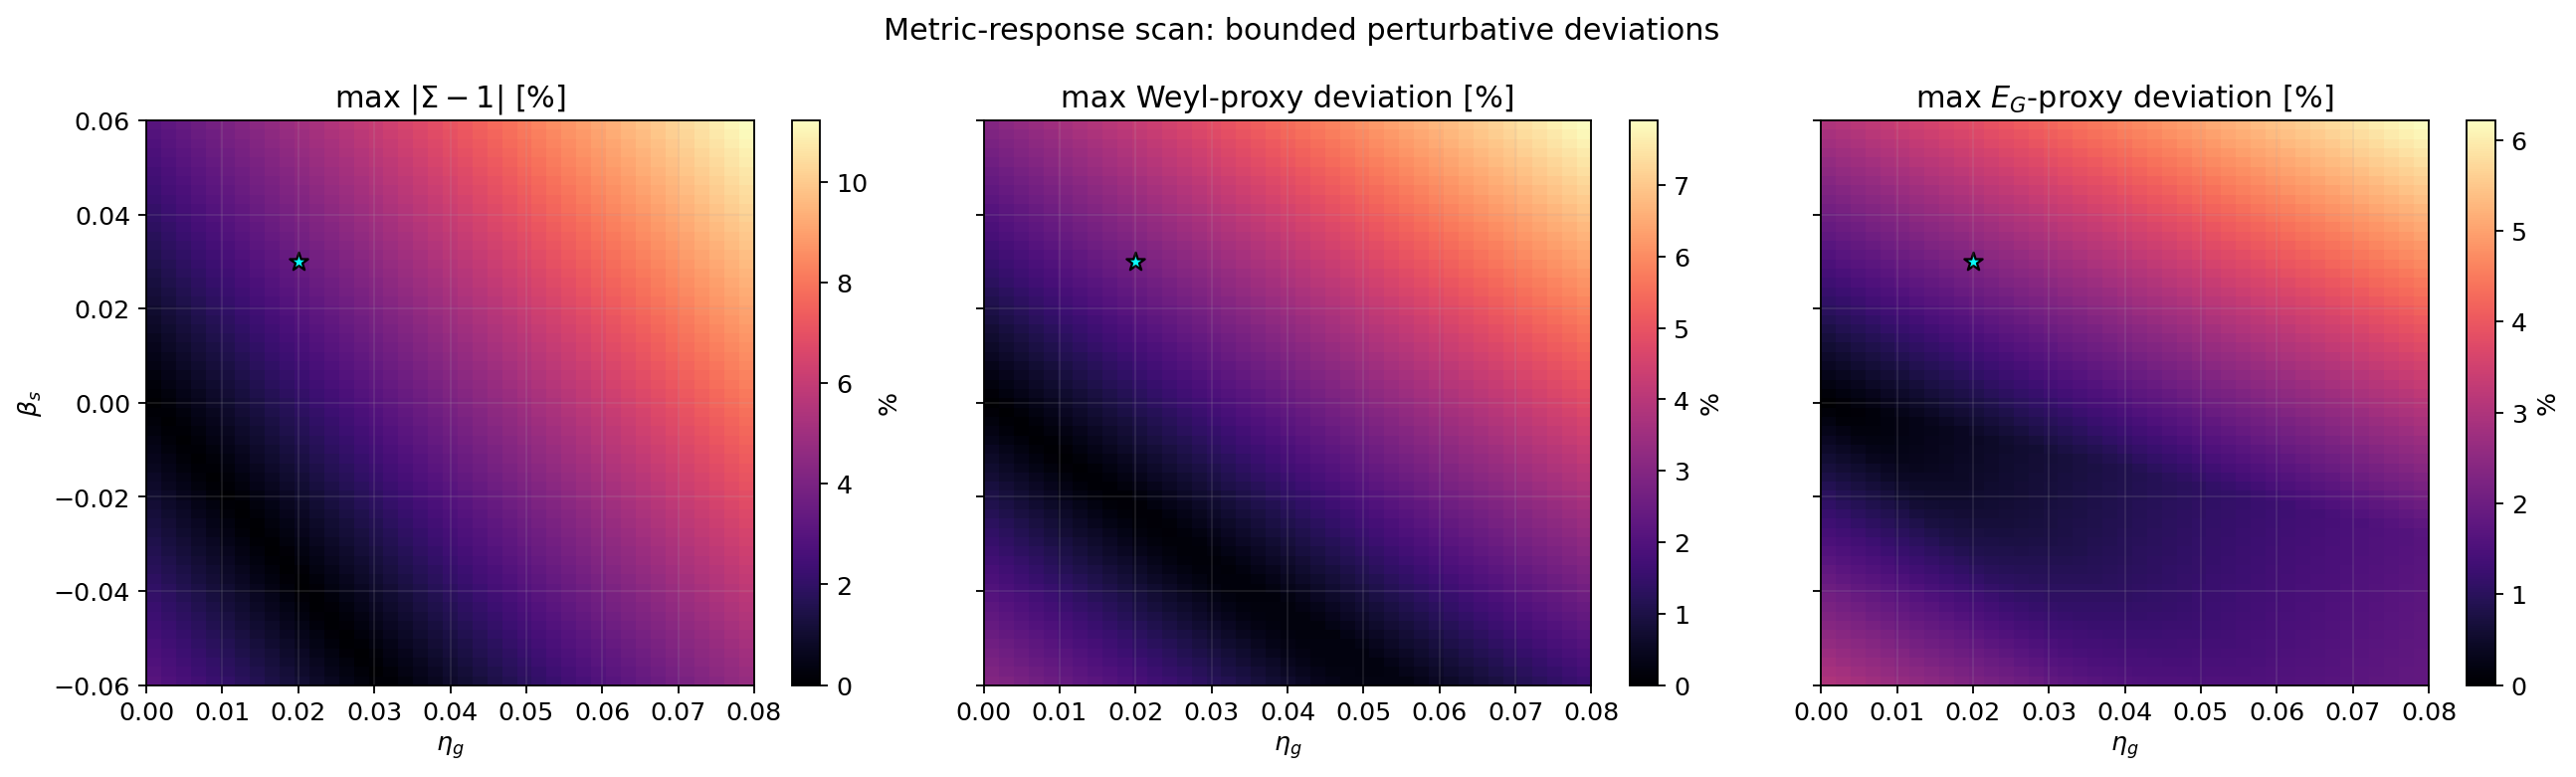
\includegraphics[width=0.98\linewidth]{fig2_metric_response_scan.png}
\caption{Metric-response scan over $(\eta_g,\beta_s)$.
The scan remains bounded and positive over the tested region.
The representative branch is marked by a star.}
\label{fig:scan}
\end{figure}

\begin{figure}[H]
\centering
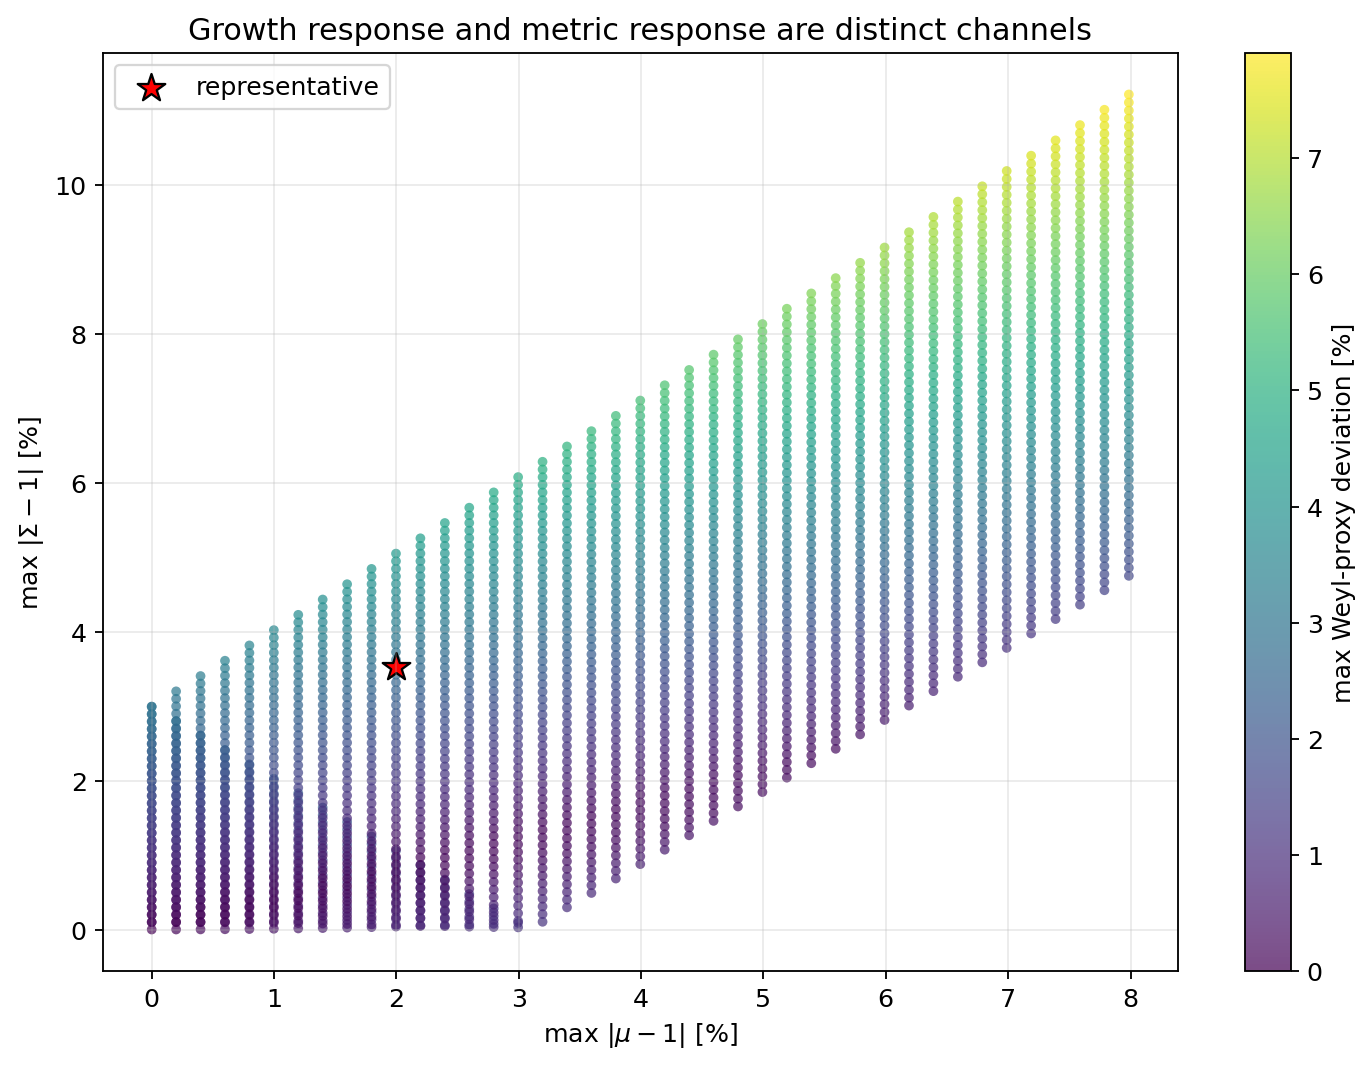
\includegraphics[width=0.82\linewidth]{fig3_growth_vs_metric_response.png}
\caption{Growth response and metric response are distinct channels.
At fixed growth coupling, changing $\beta_s$ modifies $\Sigma$ and the Weyl
proxy without changing the growth-only $\chi^2$.}
\label{fig:channels}
\end{figure}

\section{Interpretation}

Paper 45 adds the missing metric-response layer between growth-only
perturbation dynamics and future lensing-level observables.
The main conceptual result is:
\begin{quote}
\emph{MAAT projection structure can be coupled to matter growth and metric
potentials as two distinct bounded response channels.}
\end{quote}

This is important because growth data alone cannot determine whether a
structural perturbation affects only matter clustering or also the Weyl
potential.
The parameter $\eta_g$ controls the growth channel through $\mu(z)$.
The parameter $\beta_s$ controls the metric-slip channel through
$\etaslip(z)$ and $\Sigma(z)$.
This makes the two-channel structure explicit: $\eta_g$ changes the effective
source strength for matter perturbations, while $\beta_s$ changes the
relation between the two scalar potentials and therefore the Weyl/lensing
response.

In the present compact comparison, $\eta_g=0$ remains preferred by growth data,
and $\beta_s$ is unconstrained.
Thus Paper 45 is not evidence for a nonzero metric response.
Its contribution is to establish the formal bridge needed for future
weak-lensing, ISW, and growth--lensing consistency tests.

\section{Limitations}

The limitations are substantial:
\begin{itemize}[leftmargin=1.5em]
\item no Boltzmann-code implementation,
\item no CMB anisotropy calculation,
\item no weak-lensing likelihood,
\item no galaxy--lensing cross-correlation,
\item no scale dependence in $\mu(k,z)$ or $\Sigma(k,z)$,
\item no nonlinear structure formation,
\item no MCMC inference or covariance treatment.
\end{itemize}
The benchmark should be read as a reproducible effective-theory bridge, not as
a data-level cosmological constraint.

\section{Reproducibility}

The code and outputs are stored in:
\begin{center}
\texttt{experiments/maat\_metric\_response\_paper45/}
\end{center}

Run:
\begin{verbatim}
python3 maat_metric_response_solver_v01.py
\end{verbatim}

The script writes:
\begin{itemize}[leftmargin=1.5em]
\item \texttt{outputs\_paper45/paper45\_summary.json},
\item \texttt{outputs\_paper45/paper45\_metric\_curves.csv},
\item \texttt{outputs\_paper45/paper45\_metric\_scan.csv},
\item \texttt{outputs\_paper45/paper45\_growth\_metric\_comparison.csv},
\item three PNG figures used in this paper.
\end{itemize}

The public repository is:
\begin{center}
\url{https://github.com/Chris4081/structural-selection-principle}
\end{center}

\paragraph{Data attribution and license note.}
The Planck-normalised reference parameters and compact $\fsig$ comparison
points are external scientific data and should be cited to the original
publications/collaborations when reused or discussed.
The CSV tables and figures in this repository are derived reproducibility
artifacts only.
No endorsement by the Planck Collaboration, survey collaborations, or original
data authors is implied.

\section{Conclusion}

We introduced a minimal effective metric-response benchmark for MAAT
structural cosmology.
The construction extends the Paper-43 growth response
$\mu(z)=1+\eta_g\Chatproj(z)$ by adding gravitational slip
$\etaslip(z)=1+\beta_s\Chatproj(z)$ and the Weyl/lensing response
$\Sigma(z)=\mu(1+\etaslip)/2$.

All scanned branches remain positive and stable in the tested interval.
The compact growth comparison still prefers $\eta_g=0$ and cannot constrain
$\beta_s$.
For a representative nonzero branch, the metric response remains at the
few-percent level.

The next hard step is not another proxy, but a full perturbation implementation
with scale dependence and weak-lensing/CMB likelihoods.

\begin{thebibliography}{99}

\bibitem{maBertschinger1995}
C.-P.~Ma and E.~Bertschinger,
``Cosmological Perturbation Theory in the Synchronous and Conformal Newtonian
Gauges,''
\emph{Astrophys.\ J.} \textbf{455}, 7 (1995).

\bibitem{amendola2008}
L.~Amendola, M.~Kunz, and D.~Sapone,
``Measuring the dark side with weak lensing,''
\emph{JCAP} \textbf{04}, 013 (2008).

\bibitem{joyce2015}
A.~Joyce, B.~Jain, J.~Khoury, and M.~Trodden,
``Beyond the Cosmological Standard Model,''
\emph{Phys.\ Rep.} \textbf{568}, 1--98 (2015).

\bibitem{clifton2012}
T.~Clifton, P.~G. Ferreira, A.~Padilla, and C.~Skordis,
``Modified Gravity and Cosmology,''
\emph{Phys.\ Rep.} \textbf{513}, 1--189 (2012).

\bibitem{planck2018}
Planck Collaboration,
``Planck 2018 results. VI. Cosmological parameters,''
\emph{Astron.\ Astrophys.} \textbf{641}, A6 (2020).

\bibitem{alam2017}
S.~Alam et al.,
``The clustering of galaxies in the completed SDSS-III Baryon Oscillation
Spectroscopic Survey: cosmological analysis of the DR12 galaxy sample,''
\emph{Mon.\ Not.\ R.\ Astron.\ Soc.} \textbf{470}, 2617--2652 (2017).

\bibitem{kriegPaper43}
C.~Krieg,
``Linear Perturbations and Structure Growth in Structural-Selection
Cosmology,''
preprint (2026).

\end{thebibliography}

\end{document}
